% 1.2.WhenUsedCMake.tex
%	Last update: 2019/07/22 F.Kanehori
%\newpage
\subsection{CMakeを使用した場合}
\label{subsec:WhenUsedCMake}

\noindent
Cmakeは、\VS やmakeのように
ソースコードのビルドやデバッグの制御をすることを目的としたツールではなく、
ビルドの自動化を図るためのツールです。
CMakeは、\CMakeLists{}というパラメータファイルから
solution/project file (\VS)やMakefile (make)を自動的に生成します
(configureに近いものと考えていただいてよいでしょう)。

\medskip
\noindent
Cmakeはout of source (out of place)でのビルドに対応しています。
これはソースツリーの外側にビルドツリーを生成する機能で、
\Vskip{-.5\baselineskip}
\begin{itemize}
  \item	互いに干渉しない複数のビルドツリーを作成することができる。
  \item	ビルドツリーが削除されてもソースツリーに影響が及ばない。
\end{itemize}
\Vskip{-.5\baselineskip}
という特徴があります。
我々はCmakeをout of sourceで使用します。

\medskip
\noindent
ソースツリーおよびビルドツリーは次のようになるでしょう
(図\ref{fig:SpringheadLibraryTree}および図\ref{fig:ApplicationTree})。

\ifLwarp
\Vskip{-.5\baselineskip}
\begin{narrow}
    \begin{figure}[h]
	\begin{center}
	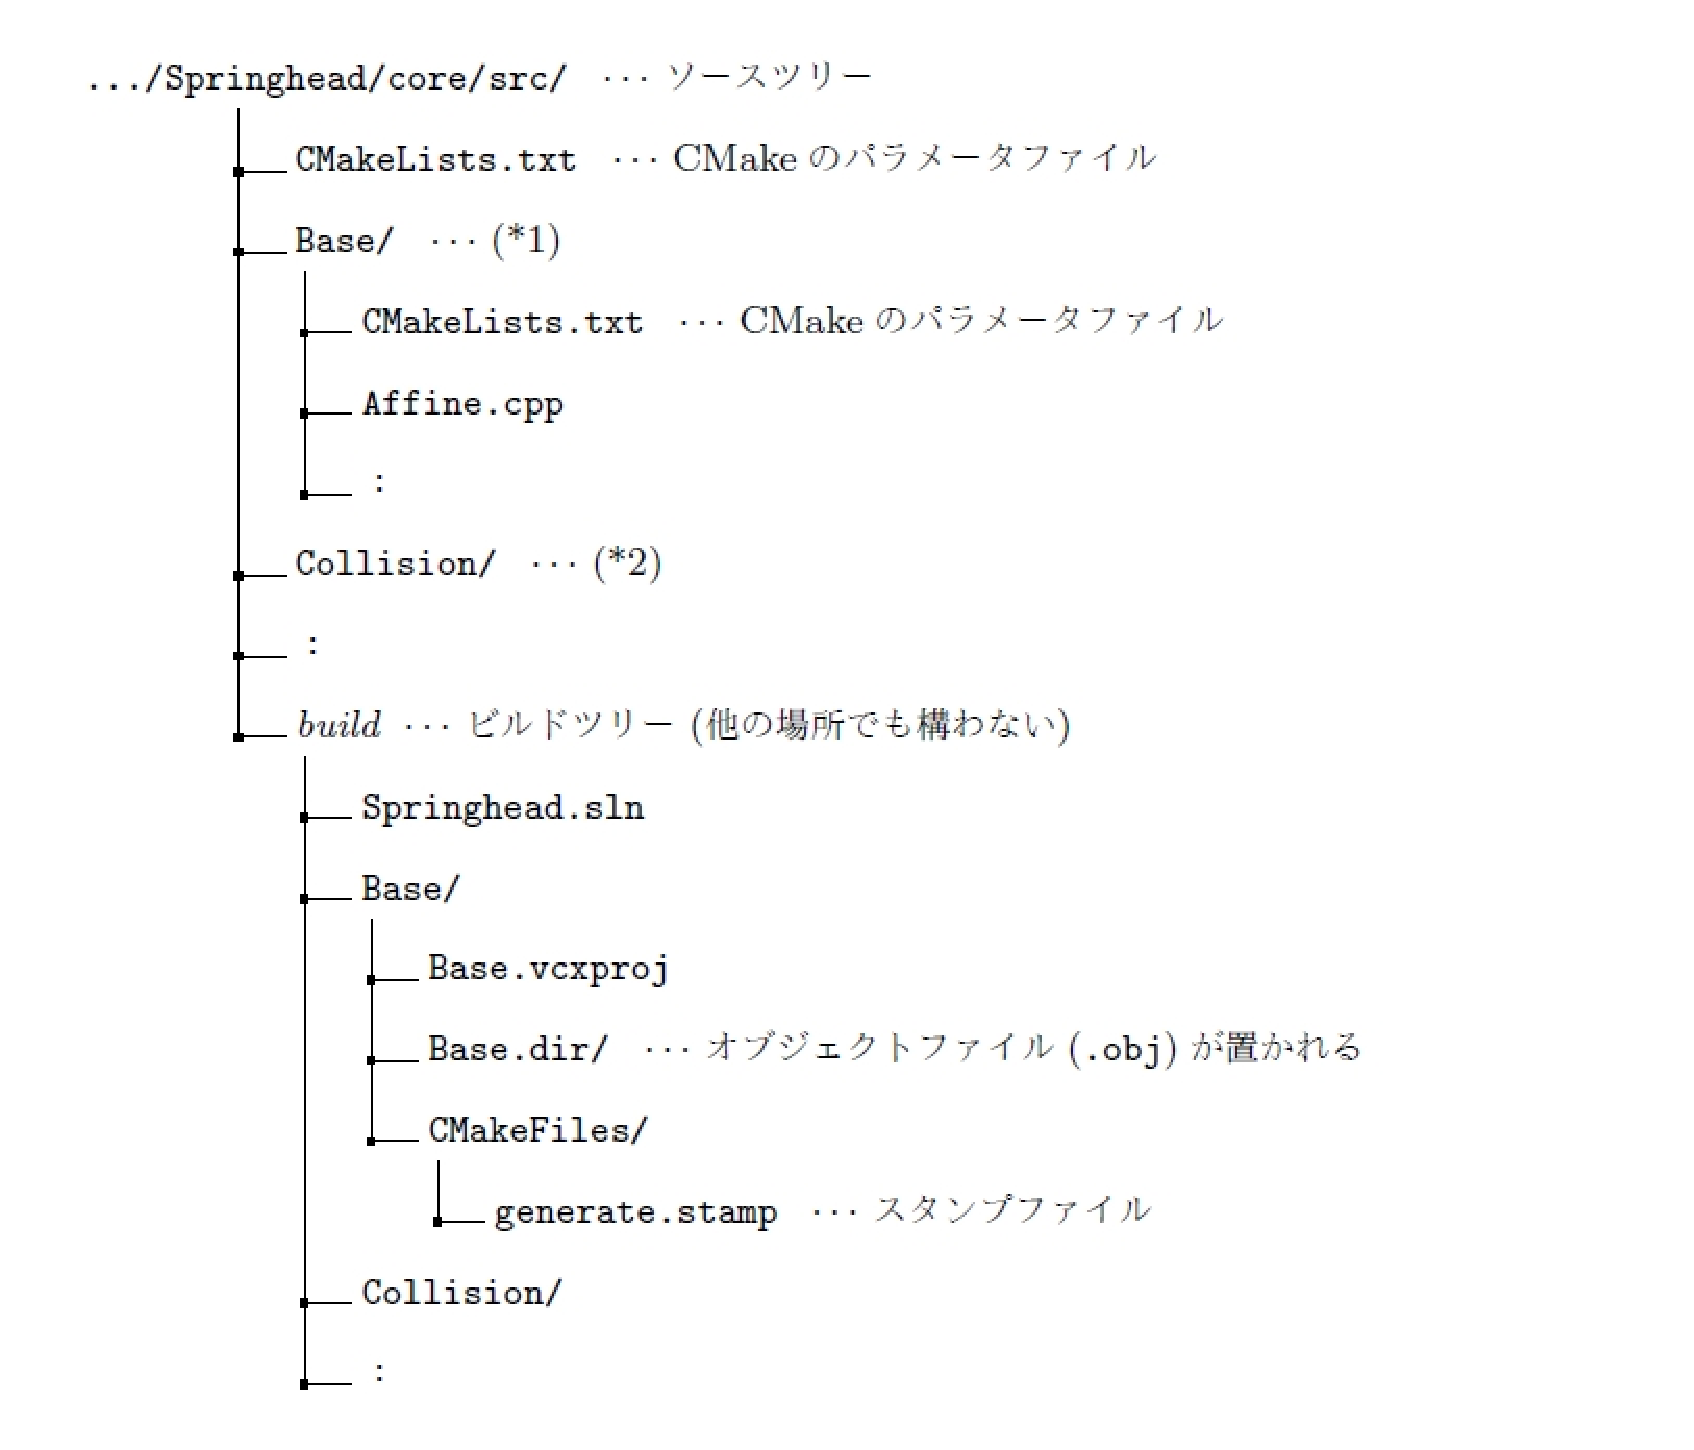
\includegraphics[width=.9\textwidth]{fig/LibraryTree.eps}
	\end{center}
	\caption{Springhead Library構成}
	\label{fig:SpringheadLibraryTree}
    \end{figure}
\end{narrow}
\else
\begin{narrow}\begin{figure}[h]
    \begin{narrow}[40pt]\begin{minipage}{\textwidth}
	{\footnotesize{\dirtree{%
		.1 \hspace{-10mm}.../Springhead/core/src/ \Anno{ソースツリー}.
		.2 CMakeLists.txt \Anno{CMakeのパラメータファイル}.
		.2 Base/ \Anno{(*1)}.
		.3 CMakeLists.txt \Anno{CMakeのパラメータファイル}.
		.3 Affine.cpp.
		.3 :.
		.2 Collision/ \Anno{(*2)}.
		.2 :.
		.2 \build \Anno{ビルドツリー (他の場所でも構わない)}.
		.3 Springhead.sln.
		.3 Base/.
		.4 Base.vcxproj.
		.4 Base.dir/ \Anno{オブジェクトファイル(\tt{.obj})が置かれる}.
		.4 CMakeFiles/.
		.5 generate.stamp \Anno{スタンプファイル}.
		.3 Collision/.
		.3 :.
	}}}
	\medskip
    \end{minipage}\end{narrow}
    \caption{Springhead Library構成}
    \label{fig:SpringheadLibraryTree}
\end{figure}\end{narrow}
\fi

\ifLwarp
\Vskip{-.5\baselineskip}
\begin{narrow}
    \begin{figure}[h]
	\begin{center}
	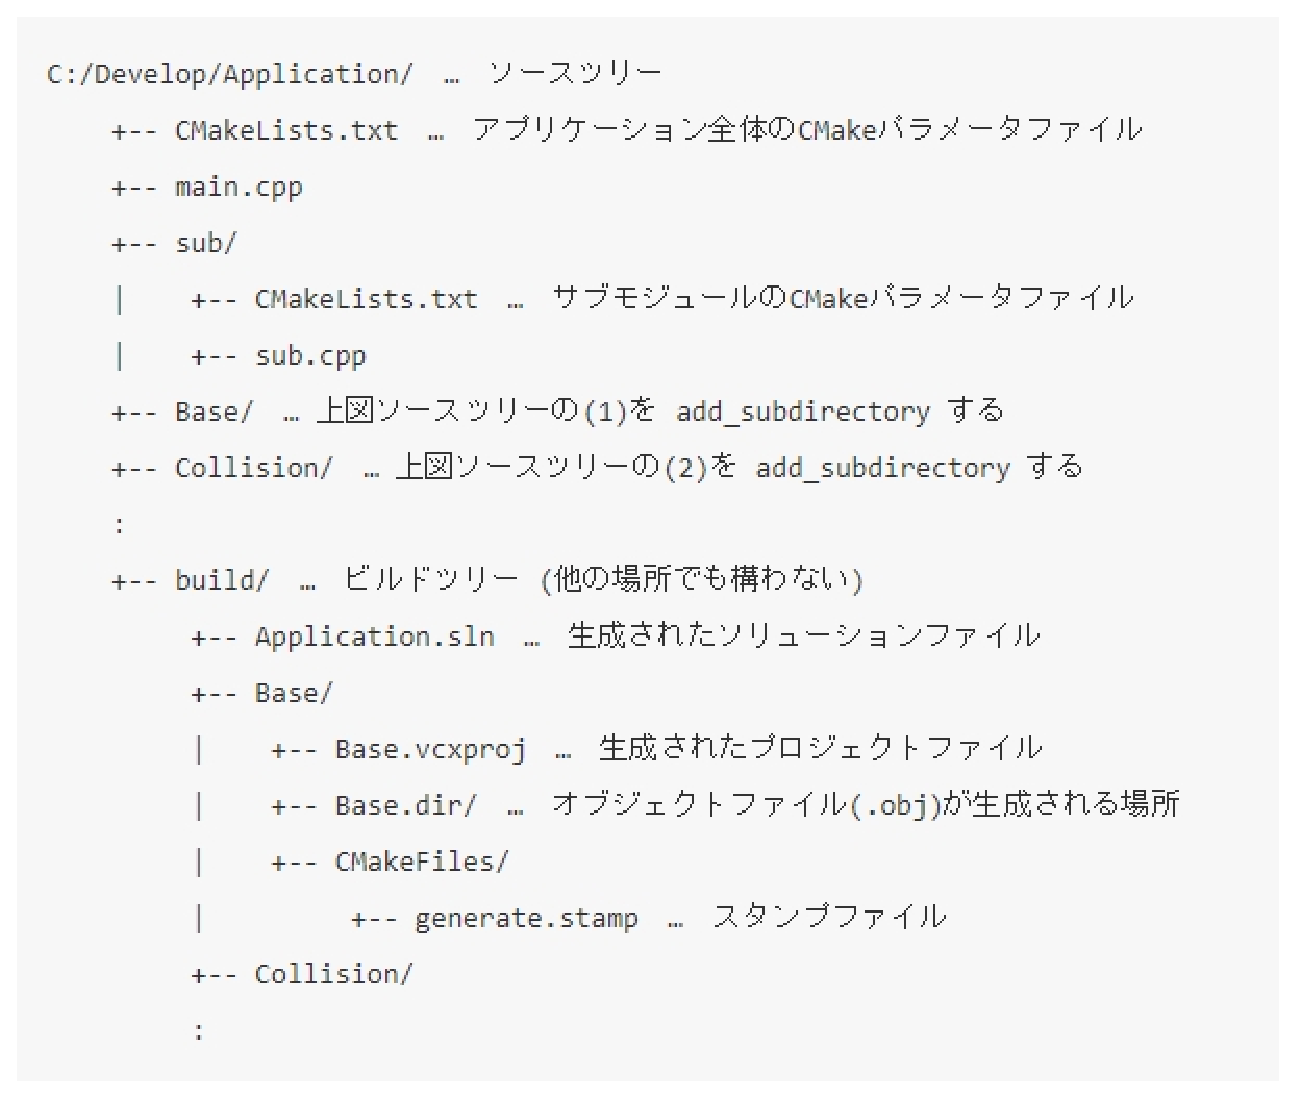
\includegraphics[width=.9\textwidth]{fig/ApplicationTree.eps}
	\end{center}
	\caption{Application構成}
	\label{fig:ApplicationTree}
    \end{figure}
\end{narrow}
\Vskip{-1.0\baselineskip}
\else
\begin{narrow}\begin{figure}[h]
    \begin{narrow}[40pt]\begin{minipage}{\textwidth}
	{\footnotesize{\dirtree{%
		.1 \hspace{-10mm}.../Application/ \Anno{ソースツリー}.
		.2 CMakeLists.txt \Anno{CMakeのパラメータファイル}.
		.2 main.cpp.
		.2 Sub/.
		.3 CMakeLists.txt \Anno{CMakeのパラメータファイル}.
		.3 sub.cpp.
		.3 :.
		.2 Base/ \Anno{Spsringheadの(*1)を指すようにする}.
		.2 Collision/ \Anno{Spsringheadの(*2)を指すようにする}.
		.2 :.
		.2 \build \Anno{ビルドツリー (他の場所でも構わない)}.
		.3 Application.sln.
		.3 Base/.
		.4 Base.vcxproj.
		.4 Base.dir/ \Anno{オブジェクトファイル(\tt{.obj})が置かれる}.
		.4 CMakeFiles/.
		.5 generate.stamp \Anno{スタンプファイル}.
		.3 Collision/.
		.3 :.
	}}}
	\medskip
    \end{minipage}\end{narrow}
    \caption{Application構成}
    \label{fig:ApplicationTree}
\end{figure}\end{narrow}
\fi

\medskip
\noindent
\CMakeLists{}はメインディレクトリおよびサブディレクトリのそれぞれに作成します。

% end: 1.2.WhenUsedCMake.tex
